\documentclass{/workdir/classes/summary}

\graphicspath{{figures/}}

% タイトルの項目
\title{和文題目}
\subtitle{和文副題} % 必要なければコメントアウト
\etitle{English Title}
\esubtitle{English Subtitle} % 必要なければコメントアウト
\studentid{00-000000}
\author{◯◯ ◯◯}
\supervisor{◯◯ ◯◯ 教授}
\abst{
    ここに100~200 word 程度の英文アブストラクト,もしくは約200文字程度の日本語概要を書く.
    ここに100~200 word 程度の英文アブストラクト,もしくは約200文字程度の日本語概要を書く.
    ここに100~200 word 程度の英文アブストラクト,もしくは約200文字程度の日本語概要を書く.
    ここに100~200 word 程度の英文アブストラクト,もしくは約200文字程度の日本語概要を書く.
    ここに100~200 word 程度の英文アブストラクト,もしくは約200文字程度の日本語概要を書く.
    ここに100~200 word 程度の英文アブストラクト,もしくは約200文字程度の日本語概要を書く.
}

\begin{document}
\maketitle

\section{序論}
本文は2段組みとする.
改行を入れて読みやすく書く.

引用例は\cite{Schlick1994}\cite{Chikushi2020}このようになる.

本文は2段組みとする.
本文は2段組みとする.
本文は2段組みとする.
本文は2段組みとする.
本文は2段組みとする.
本文は2段組みとする.
本文は2段組みとする.
本文は2段組みとする.
本文は2段組みとする.
本文は2段組みとする.
本文は2段組みとする.
本文は2段組みとする.
本文は2段組みとする.
本文は2段組みとする.

本文は2段組みとする.
本文は2段組みとする.
本文は2段組みとする.
本文は2段組みとする.
本文は2段組みとする.
本文は2段組みとする.
本文は2段組みとする.
本文は2段組みとする.
本文は2段組みとする.
本文は2段組みとする.
本文は2段組みとする.
本文は2段組みとする.
本文は2段組みとする.
本文は2段組みとする.

本文は2段組みとする.
本文は2段組みとする.
本文は2段組みとする.
本文は2段組みとする.
本文は2段組みとする.
本文は2段組みとする.
本文は2段組みとする.
本文は2段組みとする.
本文は2段組みとする.
本文は2段組みとする.
本文は2段組みとする.
本文は2段組みとする.
本文は2段組みとする.
本文は2段組みとする.

\section{提案手法}
\subsection{対象とするシステムの概要}
次のようにすべての図表は必ず本文中で引用して説明する.
\reffig{fig:logo}はロゴである.

本文は2段組みとする.
本文は2段組みとする.
本文は2段組みとする.
本文は2段組みとする.
本文は2段組みとする.
本文は2段組みとする.
本文は2段組みとする.
本文は2段組みとする.
本文は2段組みとする.
本文は2段組みとする.
本文は2段組みとする.
本文は2段組みとする.
本文は2段組みとする.
本文は2段組みとする.

本文は2段組みとする.
本文は2段組みとする.
本文は2段組みとする.
本文は2段組みとする.
本文は2段組みとする.
本文は2段組みとする.
本文は2段組みとする.
本文は2段組みとする.
本文は2段組みとする.
本文は2段組みとする.
本文は2段組みとする.
本文は2段組みとする.
本文は2段組みとする.
本文は2段組みとする.

本文は2段組みとする.
本文は2段組みとする.
本文は2段組みとする.
本文は2段組みとする.
本文は2段組みとする.
本文は2段組みとする.
本文は2段組みとする.
本文は2段組みとする.
本文は2段組みとする.
本文は2段組みとする.
本文は2段組みとする.
本文は2段組みとする.
本文は2段組みとする.
本文は2段組みとする.

本文は2段組みとする.
本文は2段組みとする.
本文は2段組みとする.
本文は2段組みとする.
本文は2段組みとする.
本文は2段組みとする.
本文は2段組みとする.
本文は2段組みとする.
本文は2段組みとする.
本文は2段組みとする.
本文は2段組みとする.
本文は2段組みとする.
本文は2段組みとする.
本文は2段組みとする.

\begin{equation}
  r = \left\{
    \begin{array}{cc}
      10   & \text{if success} \\
      - 10 & \text{if fail}    \\
      - d  & \text{else}
    \end{array}
  \right. \text{.}
\end{equation}

\begin{figure}[tb]
  \centering
  
\includegraphics[keepaspectratio, width=0.8\linewidth]{utlogo.pdf}
  \caption{ロゴ}
  \label{fig:logo}
\end{figure}

\subsection{提案手法}
本文は2段組みとする.
本文は2段組みとする.
本文は2段組みとする.
本文は2段組みとする.
本文は2段組みとする.
本文は2段組みとする.
本文は2段組みとする.
本文は2段組みとする.
本文は2段組みとする.
本文は2段組みとする.
本文は2段組みとする.
本文は2段組みとする.
本文は2段組みとする.
本文は2段組みとする.

本文は2段組みとする.
本文は2段組みとする.
本文は2段組みとする.
本文は2段組みとする.
本文は2段組みとする.
本文は2段組みとする.
本文は2段組みとする.
本文は2段組みとする.
本文は2段組みとする.
本文は2段組みとする.
本文は2段組みとする.
本文は2段組みとする.
本文は2段組みとする.
本文は2段組みとする.

本文は2段組みとする.
本文は2段組みとする.
本文は2段組みとする.
本文は2段組みとする.
本文は2段組みとする.
本文は2段組みとする.
本文は2段組みとする.
本文は2段組みとする.
本文は2段組みとする.
本文は2段組みとする.
本文は2段組みとする.
本文は2段組みとする.
本文は2段組みとする.
本文は2段組みとする.

本文は2段組みとする.
本文は2段組みとする.
本文は2段組みとする.
本文は2段組みとする.
本文は2段組みとする.
本文は2段組みとする.
本文は2段組みとする.
本文は2段組みとする.
本文は2段組みとする.
本文は2段組みとする.
本文は2段組みとする.
本文は2段組みとする.
本文は2段組みとする.
本文は2段組みとする.

\begin{figure}[t]
  \centering
  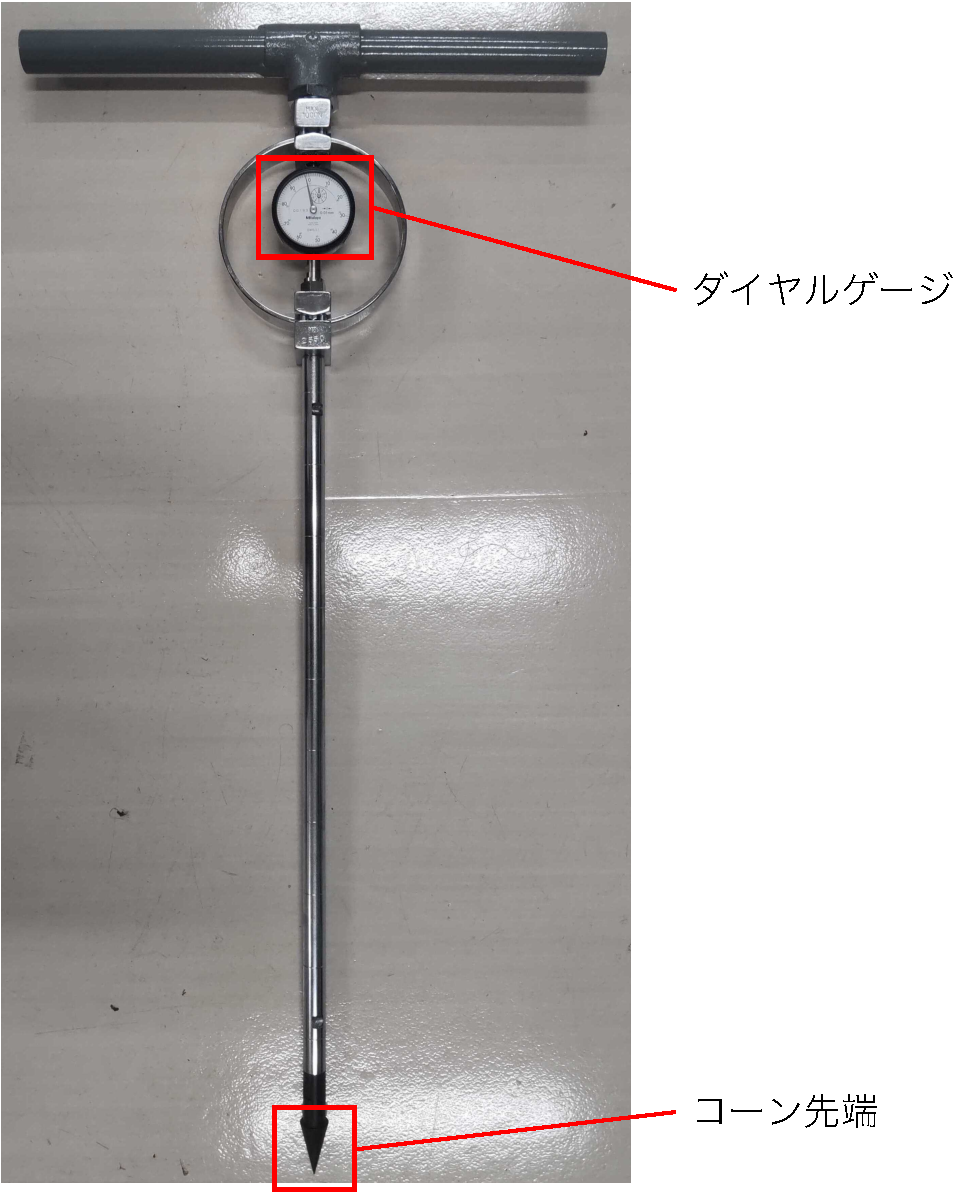
\includegraphics[keepaspectratio, width=0.5\linewidth]{chap1/cone_penetrometer.pdf}
  \caption{コーンペネトロメータ}
  \label{fig:cone_penetrometer}
\end{figure}

% textlint-disable
\begin{table}[t]
  \caption{走行に必要なコーン指数}
  \label{tab:traffic_cone_index}
  \centering
  \begin{tabular}{cc}
    \toprule
    建設機械の種類                      & コーン指数[\si{\kN/\m^2}] \\
    \midrule
    超湿地ブルドーザー                    & 200以上                \\
    湿地ブルドーザー                     & 300以上                \\
    普通ブルドーザー(\SI{15}{\tonne}級程度) & 500以上                \\
    普通ブルドーザー(\SI{21}{\tonne}級程度) & 700以上                \\
    スクレープドーザ                     & 600以上                \\
                                 & (超湿地型は400以上)         \\
    被けん引式スクレーパ(小型)               & 700以上                \\
    自走式スクレーパ(小型)                 & 1,000以上              \\
    ダンプトラック                      & 1,200以上              \\
    \bottomrule
  \end{tabular}
  \vspace{\zh}
\end{table}
% textlint-enable

\section{検証実験}
本文は2段組みとする.
本文は2段組みとする.
本文は2段組みとする.
本文は2段組みとする.
本文は2段組みとする.
本文は2段組みとする.
本文は2段組みとする.
本文は2段組みとする.
本文は2段組みとする.
本文は2段組みとする.
本文は2段組みとする.
本文は2段組みとする.
本文は2段組みとする.
本文は2段組みとする.

本文は2段組みとする.
本文は2段組みとする.
本文は2段組みとする.
本文は2段組みとする.
本文は2段組みとする.
本文は2段組みとする.
本文は2段組みとする.
本文は2段組みとする.
本文は2段組みとする.
本文は2段組みとする.
本文は2段組みとする.
本文は2段組みとする.
本文は2段組みとする.
本文は2段組みとする.

本文は2段組みとする.
本文は2段組みとする.
本文は2段組みとする.
本文は2段組みとする.
本文は2段組みとする.
本文は2段組みとする.
本文は2段組みとする.
本文は2段組みとする.
本文は2段組みとする.
本文は2段組みとする.
本文は2段組みとする.
本文は2段組みとする.
本文は2段組みとする.
本文は2段組みとする.

本文は2段組みとする.
本文は2段組みとする.
本文は2段組みとする.
本文は2段組みとする.
本文は2段組みとする.
本文は2段組みとする.
本文は2段組みとする.
本文は2段組みとする.
本文は2段組みとする.
本文は2段組みとする.
本文は2段組みとする.
本文は2段組みとする.
本文は2段組みとする.
本文は2段組みとする.

\section{実験結果・考察}
本文は2段組みとする.
本文は2段組みとする.
本文は2段組みとする.
本文は2段組みとする.
本文は2段組みとする.
本文は2段組みとする.
本文は2段組みとする.
本文は2段組みとする.
本文は2段組みとする.
本文は2段組みとする.
本文は2段組みとする.
本文は2段組みとする.
本文は2段組みとする.
本文は2段組みとする.

本文は2段組みとする.
本文は2段組みとする.
本文は2段組みとする.
本文は2段組みとする.
本文は2段組みとする.
本文は2段組みとする.
本文は2段組みとする.
本文は2段組みとする.
本文は2段組みとする.
本文は2段組みとする.
本文は2段組みとする.
本文は2段組みとする.
本文は2段組みとする.
本文は2段組みとする.

本文は2段組みとする.
本文は2段組みとする.
本文は2段組みとする.
本文は2段組みとする.
本文は2段組みとする.
本文は2段組みとする.
本文は2段組みとする.
本文は2段組みとする.
本文は2段組みとする.
本文は2段組みとする.
本文は2段組みとする.
本文は2段組みとする.
本文は2段組みとする.
本文は2段組みとする.

本文は2段組みとする.
本文は2段組みとする.
本文は2段組みとする.
本文は2段組みとする.
本文は2段組みとする.
本文は2段組みとする.
本文は2段組みとする.
本文は2段組みとする.
本文は2段組みとする.
本文は2段組みとする.
本文は2段組みとする.
本文は2段組みとする.
本文は2段組みとする.
本文は2段組みとする.

本文は2段組みとする.
本文は2段組みとする.
本文は2段組みとする.
本文は2段組みとする.
本文は2段組みとする.
本文は2段組みとする.
本文は2段組みとする.
本文は2段組みとする.
本文は2段組みとする.
本文は2段組みとする.
本文は2段組みとする.
本文は2段組みとする.
本文は2段組みとする.
本文は2段組みとする.

\section{結論}
本文は2段組みとする.
本文は2段組みとする.
本文は2段組みとする.
本文は2段組みとする.
本文は2段組みとする.
本文は2段組みとする.
本文は2段組みとする.
本文は2段組みとする.
本文は2段組みとする.
本文は2段組みとする.
本文は2段組みとする.
本文は2段組みとする.
本文は2段組みとする.
本文は2段組みとする.

本文は2段組みとする.
本文は2段組みとする.
本文は2段組みとする.
本文は2段組みとする.
本文は2段組みとする.
本文は2段組みとする.
本文は2段組みとする.
本文は2段組みとする.
本文は2段組みとする.
本文は2段組みとする.
本文は2段組みとする.
本文は2段組みとする.
本文は2段組みとする.
本文は2段組みとする.

本文は2段組みとする.
本文は2段組みとする.
本文は2段組みとする.
本文は2段組みとする.
本文は2段組みとする.
本文は2段組みとする.
本文は2段組みとする.
本文は2段組みとする.
本文は2段組みとする.
本文は2段組みとする.
本文は2段組みとする.
本文は2段組みとする.
本文は2段組みとする.
本文は2段組みとする.

\bibliographystyle{pesummary}
\bibliography{sections/reference,sections/reference_web}
\end{document}
